\documentclass[a4paper]{mwart}
\usepackage[T1]{fontenc}
\usepackage[utf8]{inputenc}
\usepackage[polish]{babel}
\usepackage{polski}

\usepackage[pdfborder={0 0 0}]{hyperref}
\frenchspacing
\setlength{\parindent}{0pt}
\usepackage{graphicx}
\usepackage[nofoot,hdivide={1cm,*,1cm},vdivide={1cm,*,1cm}]{geometry}

\author{Kamil Breczko} 
\title{Baza danych}
\date{24 października 2017}

\begin{document}

\maketitle
\thispagestyle{empty}

\newpage

\tableofcontents
\thispagestyle{empty}

\newpage
\section{Encje}
 Przy projektowaniu sprawdzarki, potrzebna jest baza danych która posiada informacje o: 
 \begin{itemize}
	\item użytkowniku;
	\item grupie, założonej przez organizatora;
	\item przynależności danego użytkowniaka do grupy;
	\item zdefiniowanym zadaniu; 
	\item listach zadań w danej grupie; 
	\item dostępnych językach programowania oraz przydzielonych testach w danym zadaniu;
	\item wysłanym rozwiązaniu oraz poprawności danego rozwiązania;
\end{itemize}
\begin{center}	
	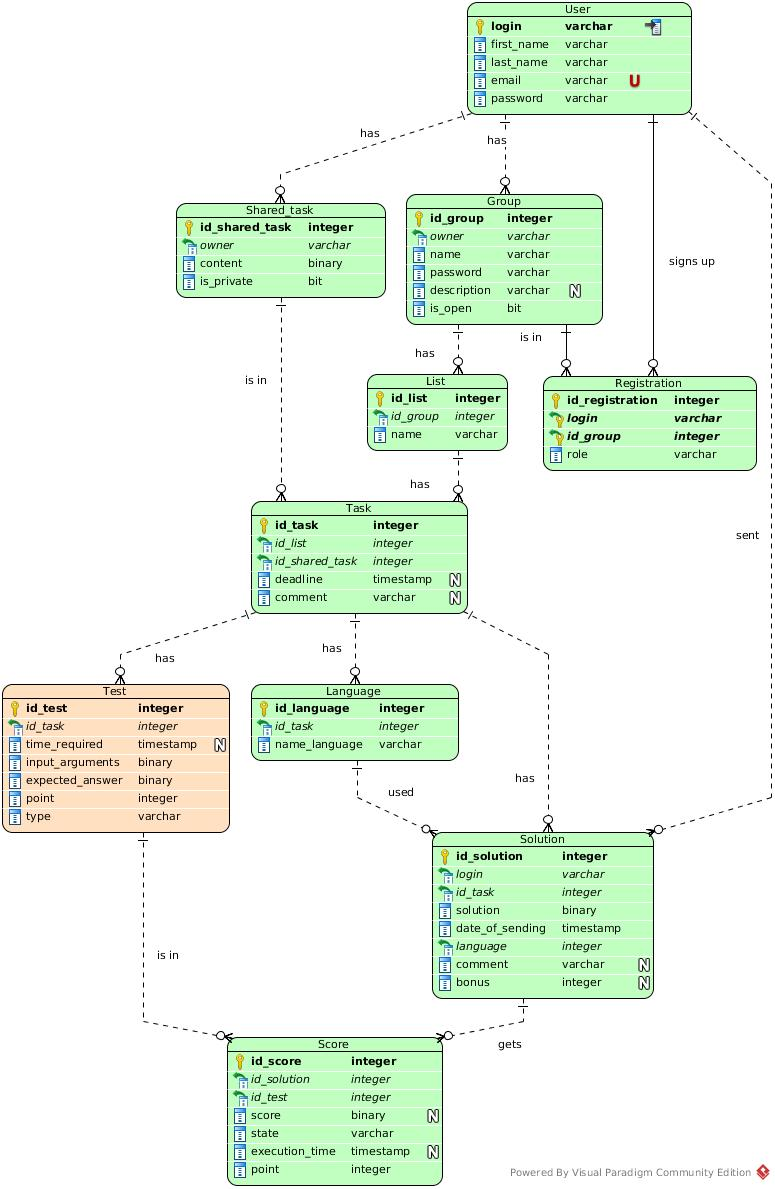
\includegraphics[scale=0.5]{diagram.jpg} \\
	Rysunek 1.1. Diagram bazy danych.
\end{center}
Dostęp do encji powinni mieć wszyscy użytkownicy, oprócz encji o nazwie \emph{Test} do której dostęp ma organizator danej grupy. 

\newpage

\section{Role}
W systemie będą istnieć trzy rodzaje użytkowników: zwykły użytkownik, organizator, administrator.

\subsection{Organizator}
Uprawnienia organizatora:
\begin{itemize}
	\item tworzenie grup ćwiczeniowych oraz zadań w danej grupie;
	\item zarządzanie stworzona grupą (nadawanie grupie hasła, zmiana nazwy, zamykanie/otwieranie grupy);
	\item dodawanie list zadań;
	\item zdefiniowanie zadania;
	\item możliwość korzystania z stworzonych zadań w innych grupach;
	\item określenie języków programowania w danym zadaniu;
	\item wstawienie testów;
	\item edycja testów;
	\item publikacja rankingu najlepszych rozwiązań;
	\item publikacja rankingu najlepszych uczestników w grupie;
	\item możliwość przydzielania dodatkowych punktów za rozwiązanie;
	\item komentowanie przesłanego rozwiązania;
	\item komentowanie zadania w danej grupie; \\
\end{itemize}

\subsection{Użytkownik}
Uprawnienia użytkownika:
\begin{itemize}
	\item zapis do istniejącej grupy;
	\item sprawdzenie wyników testów;
	\item wysyłanie programów, z określonym odstępem w czasie;
	\item wybór języka programowania;
	\item wyświetlanie rankingu najlepszych programów w zadaniu (możliwość sortowania wg. czasu i ilości zdobytych punktów za testy);
	\item przeglądanie starszych wersji rozwiązań;\\
\end{itemize}
\section{Więzy}
\subsection{Encja ,,Registration''}
Wartość w kolumnie \textit{role} może przyjmować:
\begin{itemize}
	\item user;
	\item oraganizer;
	\item administrator;
\end{itemize}

\subsection{Encja ,,Language''}
Wartość w kolumnie \textit{name\_language} powinna przyjmować nazwy języków które udostepnia sprawdzarka.

\subsection{Encja ,,Test''}
Wartość w kolumnie \textit{type} powinna przyjmować:
\begin{itemize}
	\item public -- użytkownik może wyświetlić dane wejściowe i wyjściowe;
	\item private -- użytkownik może wyświetlić tylko komunikat stanu testu;
	\item hidden -- użytkownik nie widzi testów;
\end{itemize}

\subsection{Encja ,,Score''}
Wartość w kolumnie \textit{state} może przyjmować:
\begin{itemize}
	\item TLE -- Time limit exceeded: program przekroczył limit czasu przewidziany na test;
	\item RE -- Runtime error: program zakończył się z błędem wykonania;
	\item WA -- Wrong answer: wygenerowana przez program odpowiedź jest nieprawidłowa;
	\item OK -- wygenerowana przez program odpowiedź jest poprawna;
\end{itemize}
	
\end{document}
